\documentclass[%
 reprint,
%superscriptaddress,
%groupedaddress,
%unsortedaddress,
%runinaddress,
%frontmatterverbose, 
%preprint,
%showpacs,preprintnumbers,
%nofootinbib,
%nobibnotes,
%bibnotes,
 amsmath,amssymb,
 aps,
%pra,
%prb,
%rmp,
%prstab,
%prstper,
%floatfix,
]{revtex4-1}

\usepackage{graphicx}% Include figure files
\usepackage{dcolumn}% Align table columns on decimal point
\usepackage{bm}% bold math
%\usepackage{hyperref}% add hypertext capabilities
%\usepackage[mathlines]{lineno}% Enable numbering of text and display math
%\linenumbers\relax % Commence numbering lines

%\usepackage[showframe,%Uncomment any one of the following lines to test 
%%scale=0.7, marginratio={1:1, 2:3}, ignoreall,% default settings
%%text={7in,10in},centering,
%%margin=1.5in,
%%total={6.5in,8.75in}, top=1.2in, left=0.9in, includefoot,
%%height=10in,a5paper,hmargin={3cm,0.8in},
%]{geometry}

\usepackage{cmap} % Поиск в PDF
\usepackage[T2A]{fontenc} % Кодировка
\usepackage[utf8]{inputenc} % Кодировка исходного текста
\usepackage[english, russian]{babel} % Локализация и переносы
\frenchspacing % Более тонкая настройка пробелов 
\usepackage{multirow}
\usepackage[warn]{mathtext}
\usepackage{amssymb}
\usepackage{ dsfont }
\usepackage{ textcomp }
\usepackage{ mathrsfs }

% Переопределение англоязычного начертания каппа, фи и эпсилон, 
% а также знаков сравнения
\renewcommand{\epsilon}{\ensuremath{\varepsilon}}
\renewcommand{\phi}{\ensuremath{\varphi}} 
\renewcommand{\kappa}{\ensuremath{\varkappa}}
\renewcommand{\le}{\ensuremath{\leslant}}
\renewcommand{\leq}{\ensuremath{\leqslant}}
\renewcommand{\ge}{\ensuremath{\geslant}}
\renewcommand{\geq}{\ensuremath{\geqslant}}
\renewcommand{\emptyset}{\ensuremath{\varnothing}}

\usepackage{textcomp} 
\usepackage{indentfirst} % Красная строка
\usepackage{amsmath} % Текст в формулах
\usepackage{graphicx} % Графика
\DeclareGraphicsExtensions{.pdf,.png,.jpg}
\usepackage{pgfplots}
\pgfplotsset{compat=1.13}

%\usepackage{times}

\begin{document}

\title{Изучение дифракции света}
\thanks{4.3.1}

\author{Иван Едигарьев}
\affiliation{
 Московский Физико-Технический Институт\\
 Факультет Общей и Прикладной Физики, 526т\\
}
%\date{\today}

\begin{abstract}
В работе исследуется дифракция Френеля и Фраунгофера, изучается влияние дифракции на разрешающую способность оптических инструментов.

В работе используются: оптическая скамья, ртутная лампа, монохроматор, щели с регулируемой шириной, рамка с вертикальной нитью, двойная щель, микроскоп на поперечных салазках с микрометрическим винтом, зрительная труба.

\end{abstract}

\pacs{Valid PACS appear here}

\maketitle

\begin{enumerate}

    \item 
    
    \textbf{Дифракция Френеля.}\\
    
    Сравним размер зон Френеля с измеренной шириной $D$ щели $S_2$. Для этого свяжем число тёмных полос $n$ в поле зрения с числом зон Френеля $m$ на полуширине щели. Рассчитаем величину $2 z_m$ по формуле
    \begin{gather*}
        z_m = \sqrt{a m \lambda}
    \end{gather*}
    
    и построим график $2 z_m = f(m)$. Отложим на графике величину $D$. 
    
    \begin{figure}[h]
    \center{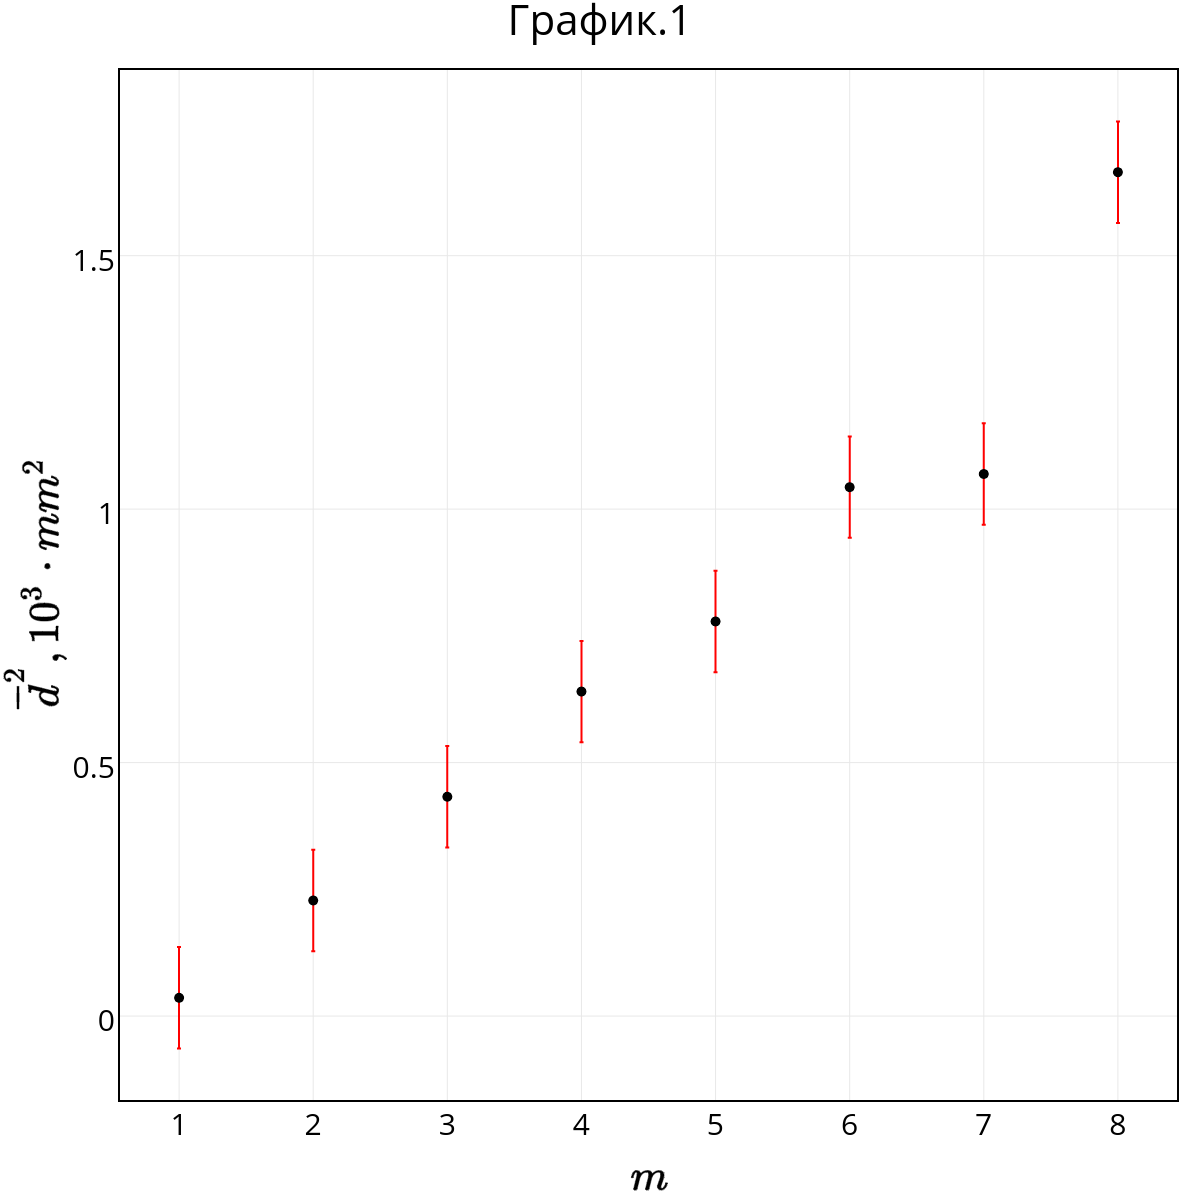
\includegraphics[scale=0.17]{my_plot1.png}}
    \end{figure}
    
    \item 

    \textbf{Дифракция Фраунгофера на щели.}\\
    
    a)  Измерим с помощью винта поперечного перемещения микроскопа координаты $x_m$ нескольких дифракционных минимумов (от $-m$ до $+m$). Определим ширину $D$ щели $S_2$ и запишем фокусное расстояние линзы $O_2$.
    
    б) Построим график, откладывая по горизонтали номер минимума $m$, а по вертикали - его координату $x_m$ (от $-m$ до $+m$). По углу наклона прямой определим среднее расстояние $\Delta x$ между соседними минимумами. 
    
    \begin{figure}[h]
    \center{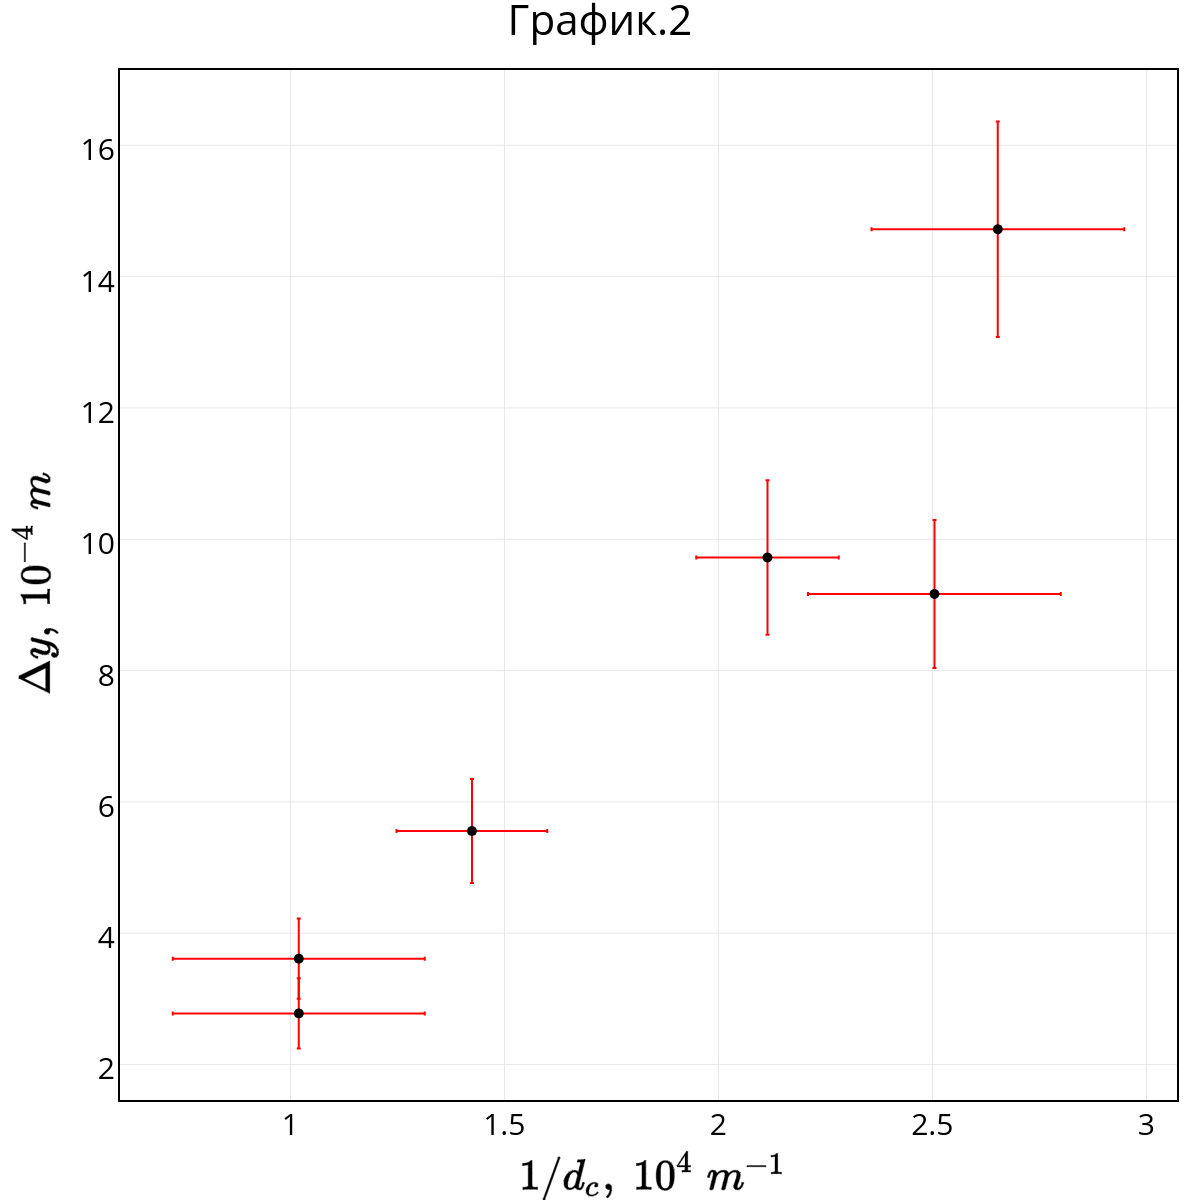
\includegraphics[scale=0.17]{my_plot2.png}}
    \end{figure}
    
    Воспользуемся методом наименьших квадратов в аппроксимации к линейной модели
    \begin{gather*}
        y = \beta x + \alpha,
    \end{gather*}
    тогда
    \begin{gather*}
        \beta = \Delta x = (260 \pm 11)~\mu m,
    \end{gather*}
    
    Рассчитаем ширину щели $D$ по формуле
    \begin{gather*}
        D = f_2 \lambda \frac{m}{x_m},
    \end{gather*}
    
    и сравним с измеренной.
    \begin{gather*}
        D^{\text{fit}} = 214~\mu m,\\
        D^{\text{изм}} = 350~\mu m.
    \end{gather*}
    
    \item 

    \textbf{Дифракция Фраунгофера на двух щелях.}\\
    
    Определим расстояние $\delta x$ между минимумами по результатам измерений
    \begin{gather*}
        \delta x = \frac{x_2 + x_1}{n} = (41 \pm 1)~\mu m.
    \end{gather*}
    
    Найдём расстояние между щелями $d$ по формуле
    \begin{gather*}
        d = f_2 \frac{\lambda}{\delta x}
    \end{gather*}
    и сравните с измеренной.
    \begin{gather*}
        d^{\text{fit}} = 1332~\mu m,\\
        d^{\text{изм}} = 1039~\mu m.
    \end{gather*}
    
    Также сравним измеренную ширину $b_0$ щели $S$ с расчётом по формуле
    \begin{gather*}
        b_0 = f_1 \frac{\lambda}{d}.
    \end{gather*}
    
    \begin{gather*}
        b_0^{\text{fit}} = (45 \pm 1)~\mu m,\\
        b_0^{\text{изм}} = 48~\mu m.
    \end{gather*}
    
    \item 
    
    \textbf{Влияние дифракции на разрешающую способность оптического инструмента.}\\
    
    Для проверки справедливости критерия Рэлея сравним измеренную ширину $D_0$ щели $S_2$ с расчётом по формуле
    \begin{gather*}
        D_0 = f_1 \frac{\lambda}{d}.
    \end{gather*}
    
    \begin{gather*}
        D_0^{\text{fit}} = (57 \pm 2)~\mu m,\\
        D_0^{\text{изм}} = 46~\mu m.
    \end{gather*}
    

\end{enumerate}

\end{document}
